\section[Data hybridization]{Aim 2 - Data hybridization for population mapping in Niger}

In 1935, British geographer Charles Fawcett defined three phenomenons that could be described on a population map \citep{fawcett_population_1935}:
\begin{enumerate}
	\item The actual number of the people within given areas
	\item The density of the population in these areas
	\item The grouping, or arrangement, of the population in space.
\end{enumerate}

Each of these elements is important to design public health programs, to plan infrastructure development or to implement quick emergency response \citep{bambas_nolen_strengthening_2005,thieren_health_2005}. Meanwhile, the lack of good quality data on populations size and locations in low resource and developing countries is well known \citep{mikkelsen_global_2015}. As a consequence, most current approaches to population mapping rely on models  aimed at mapping density surfaces \citep{linard_population_2012}. This approach makes best use of the availability of large datasets for land use and other usable covariates, and of the computational ability to interpolate these  different data sources for population distribution\citep{stevens_disaggregating_2015}. As is evident for Niger in Figure \ref{AfriPopMap}, in countries with little urbanization, and poor population data, these methods end up displaying an overlay of covariate layers more than they present a credible distribution of populations.

\begin{figure}
	\begin{center}
	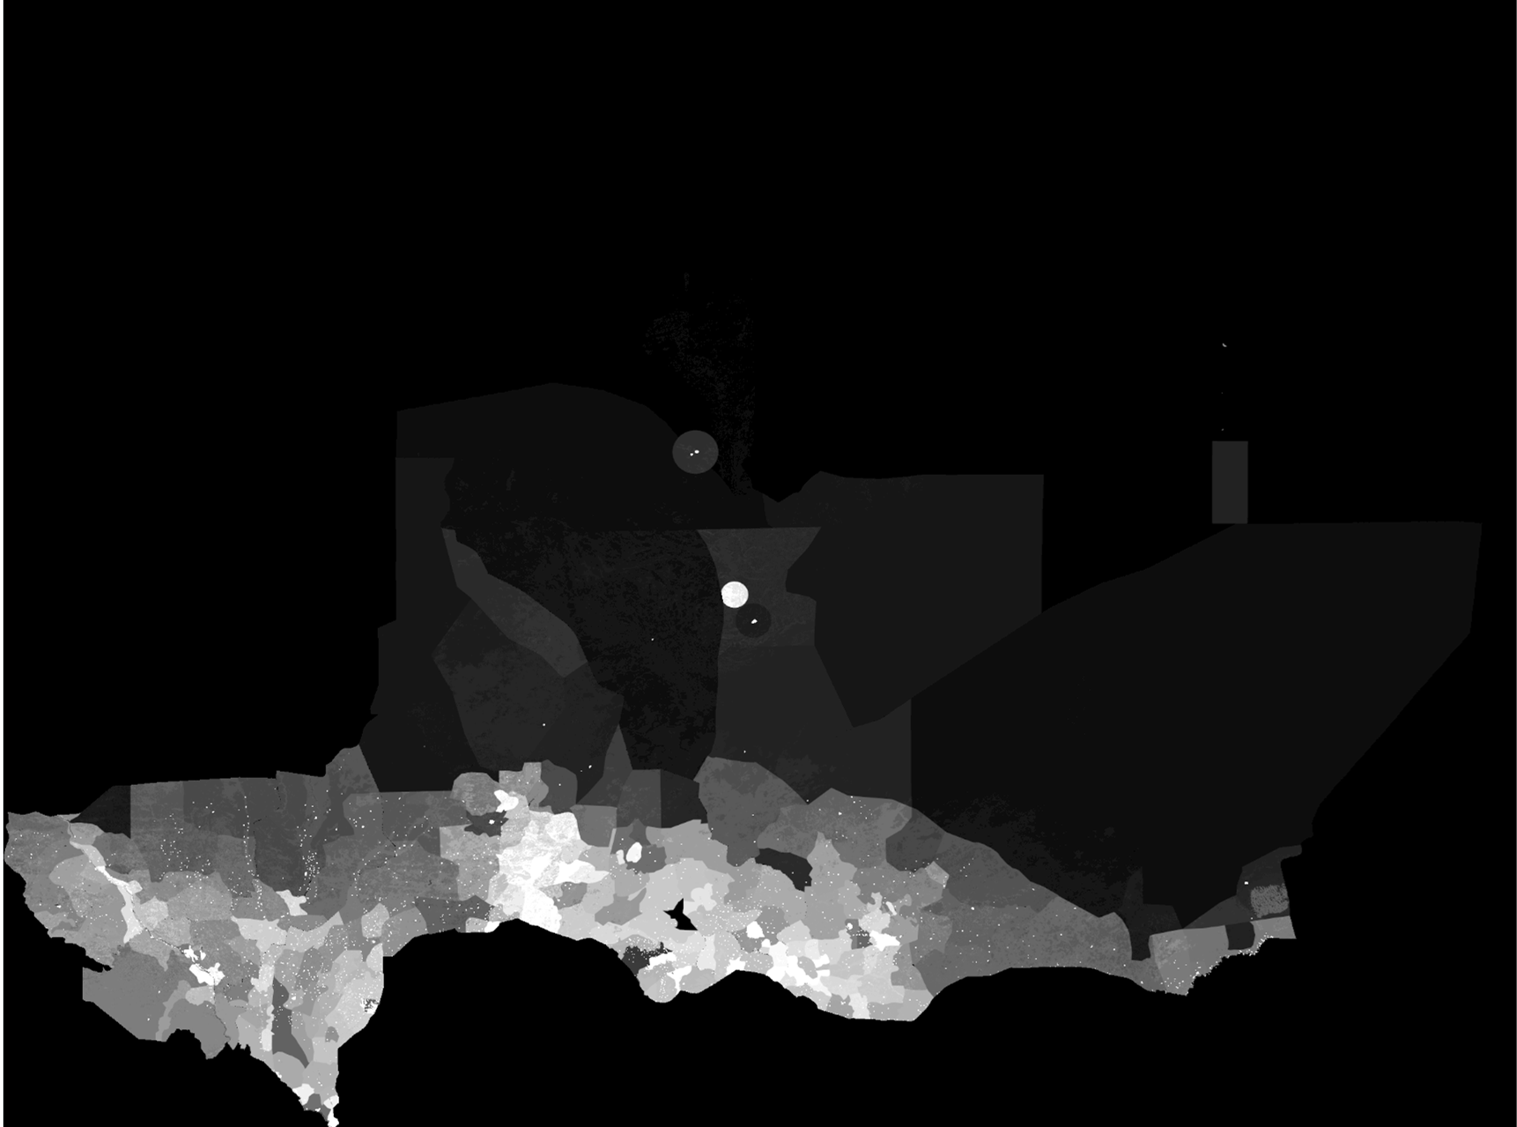
\includegraphics[width=0.8\textwidth]{figure/WORLDPOP_Niger.png}
	\caption{Mapping of Niger population from AFRIPOP}
	\label{AfriPopMap}
	\end{center}
\end{figure}

Mapping the density of the population is useful for descriptive purposes, and the production of density rasters can be essential to the spatial modeling of diseases and other population phenomenons. Meanwhile, these maps do not display actual numbers of people, nor a comprehensive display of populations groupings. Moreover, being able to query places by their name is an essential feature for managers. The information needed to produce a precise and actionable map of population in Niger can be found scattered in different unrelated data sources. This  project is exploring an innovative approach to provide a population map in Niger, through the hybridization of multiple data sources and the use of Bayesian models for administrative data.

\subsection{Data}

\paragraph{Voters list as a demographic data source} A data source that is, to my knowledge, seldom used to inform population mapping for public health purposes, is voters registration lists. There is meanwhile a case to be made for the use of voters' registration data to estimate size and the spatial distribution of populations. By definition, voters' registration should aim at being as complete as possible a register of adults in the nation. Moreover, in most democracies, some form of national elections are held at least  every five years, leading to an update at least partial of voters' registrations. In sub-Saharan Africa, between the years 2015 and 2016, 27 countries were supposed to hold national elections, leading to a theoretical registration of more than half of the adult population of the continent. Finally, for transparency and accountability reasons, electors registries are supposed to be accessible.

Due to the sensitive and political use of these data, the quality of voters registries are often described as not being trustworthy. On the other hand, for the same sensitivity reasons, voters registries are receiving a high level of scrutiny from different actors, and are audited sometimes multiple times before validation. This level of scrutiny before validation is much higher than the attention given to a lot of studies or other often used data sources.

\paragraph{The Niger 2016 elections voters registry} In Niger, presidential and parliamentary elections were held in February 2016. Voters lists were updated during the second half of the year 2015, under the supervision and control of a mission of the \gls{oif}. The operations for registration of voters were conducted during the third quarter of 2015\footnote{\url{http://www.ceni-niger.org/article-region/##more-24}}.
A first version of the voters list was published on December 21, 2015, tallying 7,569,172 voters, out of 8,569,309 that were expected based on the 2012 census\footnote{\url{http://www.iinanews.org/page/public/news_details.aspx?id=98929&NL=True}}

Final lists were validated in early January 2016 after being corrected for some incoherencies noted by the supervisory body\footnote{\url{http://www.nigerinter.com/2016/01/le-fichier-electoral-du-niger-valable-sous-reserves/}}.
A final report on these lists was published in may 2016\footnote{\url{http://www.nigerinter.com/2016/05/remise-officielle-du-rapport-du-fichier-electoral-au-ministre-detat-a-linterieur-par-le-cfeb/}}.
The \gls{ceni} later made these lists fully available on its website, from which I extracted, anonymized and formatted the lists.

\paragraph{RENALOC and RENACOM} The \gls{renaloc} is a geolocalized repertory of all localities in Niger.  The 2012 version was downloaded as a pdf file from the \gls{ins} website. The tables were extracted in bulk from this file using the Tabula Package, and then processed in Python to recompose the geographic structure of the document. The final data consists in 34507 localities, for which the INS provides the number of inhabitants, by gender, as well as the number of households, and the number of agricultural households. For most of the localities, a GPS coordinate is recorded, as well as the type of locality (neighborhood, village, camp, water well, hamlet).

The 2001 version of this database, named \gls{renacom}, contains similar information. Meanwhile, the number of places identified varies, and for places identified in \gls{renaloc} and \gls{renacom}, some names spelling vary. I retrieved the \gls{renacom} in Excel tabular format directly from the \gls{ins} website.

\paragraph{OpenStreetMap} \gls{osm} is "a free, editable map of the whole world that is being built by volunteers largely from scratch and released with an open-content license"\footnote{\url{http://wiki.openstreetmap.org/wiki/About_OpenStreetMap}}. Its API allows an easy query of its content, from which we can retrieve places names and community generated GPS coordinates. This data can provide additional precisions on where some localities are, but is much less complete than both \gls{renaloc} and \gls{renacom}.

\paragraph{DHI2} The Niger \gls{snis} is currently implementing \gls{dhis2}. The portal to \gls{dhis2} already makes available some limited geolocalization data, regarding the health districts divisions, and some health facilities coordinates\footnote{\url{http://www.snisniger.ne/dhis-web-commons/security/login.action}}.


\subsection{Methods}

To make the best use of this data, I will implement an approach based on a minimal modelling of primary population data, and geared towards the anchoring of population in callable named localization. To achieve this, my project has three main components.

\subsubsection{Name Matching}

Due to the history of the creation and administration of the Nigerien territory, multiple different spellings are in use for most localities names in Niger. There are no obvious reasons to prioritize one spelling over another for this project. To the contrary, I want users to be able to use whichever spelling of a name they prefer to query their results.

In collaboration with Fahad Pervaiz, a PhD student in the department of Computer Science at UW, I am designing a matching algorithm for different spellings of the same locality names in Niger. Our approach relies on the use of  a mixture of standard string matching algorithms. We use these algorithms for each pair of data sources and define a heuristic to combine them and select best matches. We also enrich these heuristics by defining patterns and features that allow a first classification and simplification of names to improve matching performance. These patterns may be data source specific to reflect explicit or non-explicit conventions used in each data source.

After this first round of unsupervised matching, we will manually confirm some of the matches with the help of members of the \gls{osm} community in Niger. Using this validated training set, we will fit supervised algorithms to improve our previous matching approach.

As a result of this step, I will have a consolidated list of localities in Niger, with different possible spellings of names for each of them.

\subsubsection{Locality mapping}

The three data sources that include GPS coordinates (\gls{renaloc}, \gls{renacom}, \gls{osm}) have GPS coordinates for different subsets of localities in Niger. It appears that \gls{renaloc} GPS coordinates are of very low quality, and that \gls{osm} coordinates are sometimes rough estimates of exact locations with a rounding factor. I will design an algorithm to attach, for each identified locality, the most probable GPS localization.

\begin{enumerate}
\item Get \gls{renacom} GPS coordinates for localities where they are available.
\item Fit some models to correct GPS coordinates in gls{renaloc} using localities with both \gls{renaloc} and \gls{renacom} GPS coordinates. Use the best performing approach, as evaluated with cross-validation, to correct RENALOC coordinates
\item Fit some models to correct GPS coordinates in \gls{osm} using localities with both \gls{osm} and \gls{renacom} GPS coordinates. Use the best performing approach, as evaluated with cross-validation, to correct \gls{osm} coordinates
\end{enumerate}

For steps 2 and 3, different linear models will be tested, as well as non linear Machine Learning approaches allowing for different local corrections. For localities with \gls{renaloc} and \gls{osm} coordinates but no \gls{renacom}, I will evaluate if the results 2 or 3 or a combination of both performs best, using localities with GPS from the three data sources as training set.

As a result of this step, I will have the most complete and accurate grid possible of named localities in Niger.

\subsubsection{Population modeling}

Finally, I will model Niger population using its voters list by voting precinct as a main data source. I could not source an example of using voters list as a source for demographic estimation. Meanwhile, in a country like Niger where elections are held much more regularly than censuses, using voting lists, a quasi complete enumeration of the population, to estimate population size and structure, does not seem unreasonable.

\begin{figure}[ht]
	\begin{center}
		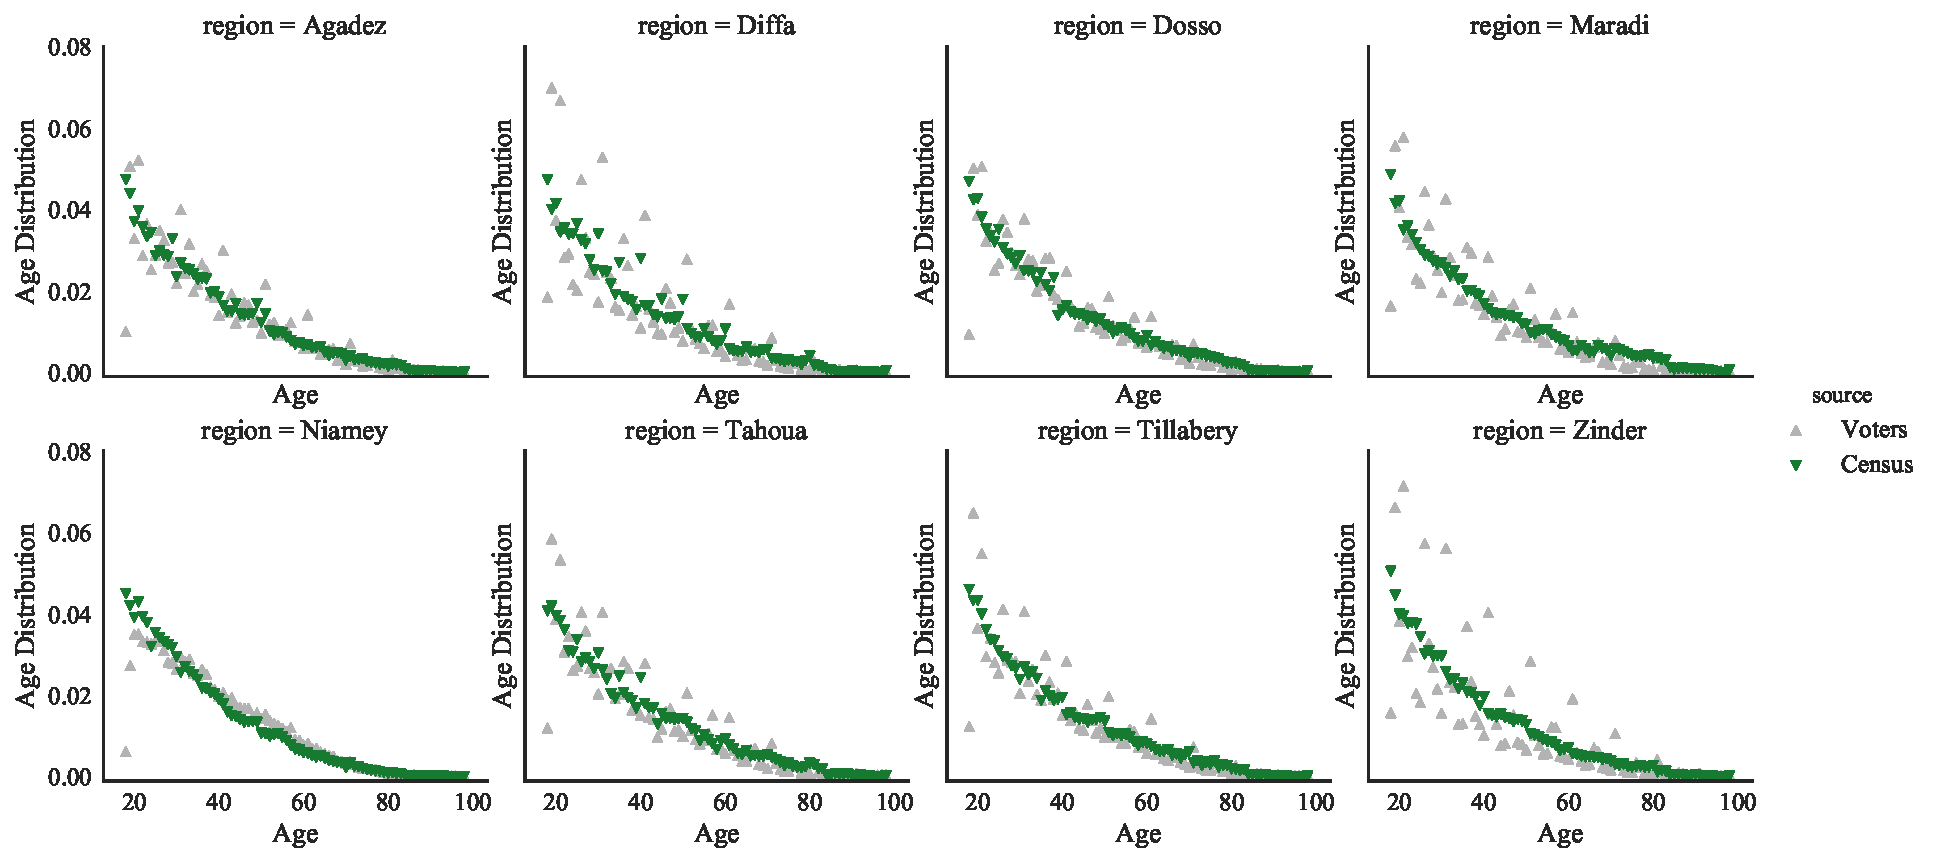
\includegraphics[width=\textwidth]{figure/age_structure_comparison.pdf}
		\caption{Comparison of standardized adult age distribution between the 2012 census and the 2016 voting lists}
		\label{fig:age_comparison}
	\end{center}
\end{figure}

A specificity of the voting list is that it does not include children under 18, as they are not allowed to vote. Additionally, the completeness of the data is not perfect, and I should assess and correct voters lists counts to correct this. Finally, as voting lists are very local, I will need to determine the most appropriate level of aggregation to get a meaningful estimation of the population age and gender distribution. Figure \ref{fig:age_comparison} compares the standardized age distribution of adults in the 2012 census and in the 2016 voters list at regional level. We can see there is more variability in the voters lists age structure than in the census. Concordance between the two age distributions seems to vary between regions.

I will model population size and age and gender distribution at regional and health zone level, using the electoral lists as input data, and the 2012 census regional distributions of population by age and gender as validation data. A simple approach will be used to keep this part of the project tractable, and easily reproducible locally. Age distributions from the voters lists will be aggregated at the regional or health zone level, and a number of children will be computed using widely available life tables. I will use multiple life tables to get an estimation of uncertainty on this estimation. The total population numbers will then be modeled in a linear regression framework, using the 2012 census numbers as validated results.

\subsection{Output}

The output of the project will  be an interactive map, allowing the query of our results for local practitioners. This dashboard will have the following feature :
\begin{enumerate}
	\item An interactive map of Niger localities, selectable by clicking, or panning for multiple selection
	\item An estimation of the population in the zone selected on the map
	\item A histogram representing the age structure of the population in the localities selected on the map
	\item A search box through which the user will be able to search for a given locality with different spellings. Every name linked to a mapped locality will be searchable and will return the different matching localities in a hierarchized way.
\end{enumerate}



\subsection{Timeline}
\label{timeline:aim2}
I am currently trying to obtain more detailed census data from Niger Census. Meanwhile, the name matching and locality mapping work is already well advanced as we have a first set of matched names from the unsupervised approach, and I have already explored approaches to GPS correction for \gls{renaloc}. I anticipate three more months on the name matching and one month to confirm the locality mapping and the overlay with other \textit{adhoc} layers such as health services and health administration map, and should have completed mapping data by September 2017. I plan 5 months of work for the population estimation, and should have my final results by February 2018. Figure \ref{GanttPaper3} summaries this timeline.

\begin{figure}[t]
	\begin{ganttchart}[vgrid,hgrid,
	y unit chart=.6cm]{1}{18}
		\gantttitle{2017}{12}
		\gantttitle{2018}{6} \\
		\gantttitlelist{1,...,12}{1} \gantttitlelist{1,...,6}{1}\\

		\ganttset{bar/.append style={draw=green!40 , fill=green!40},
                    group/.append style={draw=green, fill=green}}
		\ganttbar{Data Extraction}{1}{3} \\
		\ganttbar{Name Matching}{1}{6} \\
		\ganttbar{Locality Mapping}{7}{9} \\
		\ganttmilestone{First complete map}{9} \\
		\ganttbar{Population Estimation}{10}{14} \\
		\ganttmilestone{Sharing Final Results}{14} \\
		\ganttbar{Paper Writing}{15}{16} \\
		\ganttbar{Dashboard Design}{15}{16} \\
		\ganttmilestone{Paper Submission}{16}
	\end{ganttchart}
	\caption{Gantt Chart for Aim 3}
	\label{GanttPaper3}
\end{figure}
